\documentclass[12pt,a4paper,openright,twoside]{book}
\usepackage[utf8]{inputenc}
\usepackage{disi-thesis}
\usepackage{code-lstlistings}
\usepackage{notes}
\usepackage{shortcuts}
% \usepackage{acronym}

\school{\unibo}
\programme{Corso di Laurea in Ingegneria e Scienze Informatiche}
\title{OpenGL e Vulkan: un caso di studio}
\author{Palazzini Luca}
\date{\today}
\subject{Computer Graphics}
\supervisor{Prof.ssa Damiana Lazzaro}
\session{I}
\academicyear{2024-2025}

% Definition of acronyms
% \acrodef{API}{Application Programming Interface}
% \acrodef{PBR}{Physically Based Rendering}
% \acrodef{CPU}{Central Processing Unit}
% \acrodef{GPU}{Graphical Processing Unit}

\mainlinespacing{1.241}

\begin{document}

\frontmatter\frontispiece

% TODO: Write abstract
\begin{abstract}	
   Max 2000 characters, strict.
\end{abstract}

% TODO: Write dedication (optional)
\begin{dedication}
   Optional. Max a few lines.
\end{dedication}

% Table of contents
\tableofcontents   
\listoffigures
% TODO: Uncomment when listing added \lstlistoflistings

% Main content
\mainmatter

%----------------------------------------------------------------------------------------
\chapterWithoutNumber{Introduzione}
\label{chap:introduzione}
%----------------------------------------------------------------------------------------

\paragraph{Contesto e Motivazioni}
Negli ultimi anni, il campo della grafica computazionale ha visto un'evoluzione significativa delle \emph{Graphics APIs}
verso modelli di programmazione più vicini all'hardware e orientati alle alte prestazioni.
Lo scopo di questo elaborato è indagare le differenze prestazionali e architetturali tra due API principali,
OpenGL e Vulkan, attraverso la realizzazione di un motore di rendering capace di utilizzare entrambe le tecnologie.
Il confronto si concentra in particolare sull'impatto del multithreading in Vulkan rispetto al modello single-thread
tipico di OpenGL, analizzando come la differente gestione della pipeline grafica influisca sulle prestazioni complessive.

\paragraph{Obiettivi}
L'obiettivo principale del lavoro è progettare e sviluppare un motore di rendering scritto in \emph{C++23},
in grado di operare sia con OpenGL 4.6 sia con Vulkan 1.4.
Il motore implementa un approccio di tipo \emph{deferred rendering}, supporta materiali Physically Based Rendering (PBR),
luci direzionali, puntuali e spot, e include ulteriori passaggi di rendering per particelle e oggetti di debug.
L'architettura segue un paradigma orientato agli oggetti, integrando librerie e framework comuni.
L'obiettivo sperimentale è valutare, a parità di contenuto e condizioni di rendering, l'efficienza delle due API
in termini di:
\begin{itemize}
   \item tempo medio per frame e frame rate;
   \item utilizzo della CPU e della GPU.
\end{itemize}

\paragraph{Metodologia di lavoro}
Il progetto è stato sviluppato con un approccio incrementale, secondo cicli iterativi di implementazione e validazione.
Dopo la fase di progettazione architetturale, il motore è stato realizzato con un sistema modulare che separa la logica
di rendering dal resto della gestione della scena, consentendo di confrontare in modo diretto i due backend grafici.
I test prestazionali sono stati condotti su una scena principale: la cattedrale di Sponza~\cite{sponza_original,sponza_intel2022},
utilizzando diversi hardware, variando numero di luci e \emph{particle systems}, per misurare in modo oggettivo i benefici derivati
dal parallelismo offerto da Vulkan.

\paragraph{Struttura del documento}
Il documento è organizzato come segue:
\begin{itemize}
   \item Il \textbf{Capitolo 1} introduce i concetti fondamentali relativi al rendering, alle API grafiche moderne e alle tecniche PBR e deferred rendering;
   \item Il \textbf{Capitolo 2} analizza i requisiti del progetto e le scelte progettuali alla base del motore sviluppato;
   \item Il \textbf{Capitolo 3} descrive l'architettura del sistema e i principali componenti software;
   \item Il \textbf{Capitolo 4} illustra l'implementazione e mostra esempi di codice e schermate del motore in funzione;
   \item Il \textbf{Capitolo 5} presenta la valutazione sperimentale, i risultati delle misure e la loro analisi critica.
\end{itemize}

%----------------------------------------------------------------------------------------
\chapter{Fondamenti Teorici}
\label{chap:fondamenti-teorici}
%----------------------------------------------------------------------------------------
\noindent
Questo capitolo fornisce il quadro teorico necessario alla comprensione del lavoro svolto.
Vengono introdotti i concetti fondamentali relativi alla pipeline di rendering,
analizzando le differenze tra i principali approcci utilizzati nei motori grafici moderni,
in particolare il \emph{forward rendering} e il \emph{deferred rendering}.
Segue un approfondimento sui principi del \emph{Physically Based Rendering} (PBR),
che costituisce la base fisica dei modelli di illuminazione implementati nel motore sviluppato.
Infine, vengono presentate le due API grafiche oggetto dello studio, OpenGL e Vulkan,
e le principali librerie di supporto utilizzate nel progetto.
L’obiettivo del capitolo è fornire al lettore una visione d’insieme dei fondamenti teorici e tecnologici
su cui si basa l’intero lavoro sperimentale.

\section{Pipeline di Rendering}
Il processo di rendering di una scena tridimensionale può essere realizzato attraverso approcci differenti,
ognuno con vantaggi e limiti specifici. I due modelli principali sono il \emph{forward rendering} e il
\emph{deferred rendering}, che differiscono per il modo in cui gestiscono il calcolo dell'illuminazione e la
composizione finale dell'immagin.
Il rendering di una scena tridimensionale consiste nel trasformare modelli matematici di oggetti e luci in un'immagine bidimensionale. Questo processo può essere realizzato mediante diverse pipeline, ciascuna con vantaggi e svantaggi specifici.
Nel \emph{forward rendering}, ogni oggetto della scena viene renderizzato direttamente con tutte le luci che lo influenzano.
Durante il passaggio di rendering, per ogni frammento vengono calcolati il colore finale e il contributo luminoso
di ciascuna sorgente, con il risultato che il numero di calcoli cresce proporzionalmente al numero di luci.
Questo metodo è relativamente semplice da implementare, ma può diventare inefficiente in scene complesse, dove molte
luci influenzano simultaneamente la stessa area. Tuttavia, rimane ancora oggi una soluzione adatta a contesti con un
numero limitato di luci dinamiche o in applicazioni dove la compatibilità e la semplicità di implementazione sono prioritarie.
Il \emph{deferred rendering}, invece, suddivide il processo di rendering in più passaggi. Nel primo, chiamato
\emph{geometry pass}, vengono memorizzate nei cosiddetti \emph{G-buffer} le informazioni geometriche necessarie,
come la posizione dei punti, le normali delle superfici e le proprietà dei materiali.
\begin{figure}
   \centering
   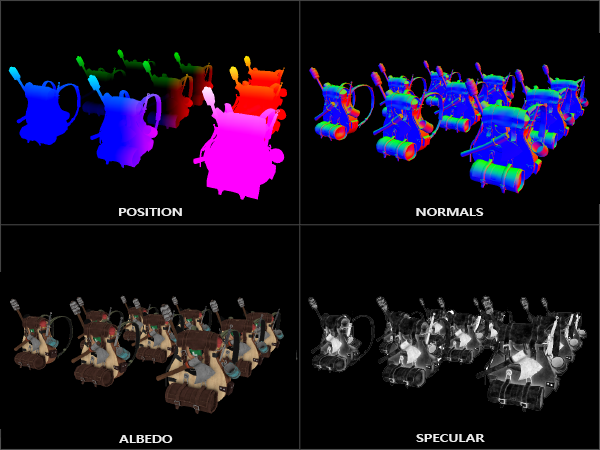
\includegraphics[width=.8\linewidth]{figures/g_buffer_example.png}
   \caption{Esempio di G-buffer in una pipeline di deferred rendering da \cite{learnopengl}.}
   \label{fig:g-buffer-example}
\end{figure}
Nel secondo passaggio, denominato \emph{lighting pass}, l'illuminazione viene calcolata utilizzando i dati salvati nei buffer,
evitando di dover eseguire nuovamente le trasformazioni geometriche per ogni luce. Questo approccio permette di gestire
un numero elevato di luci in modo più efficiente, rendendolo particolarmente indicato per applicazioni moderne e motori
di gioco con scenari complessi.
\begin{figure}
   \centering
   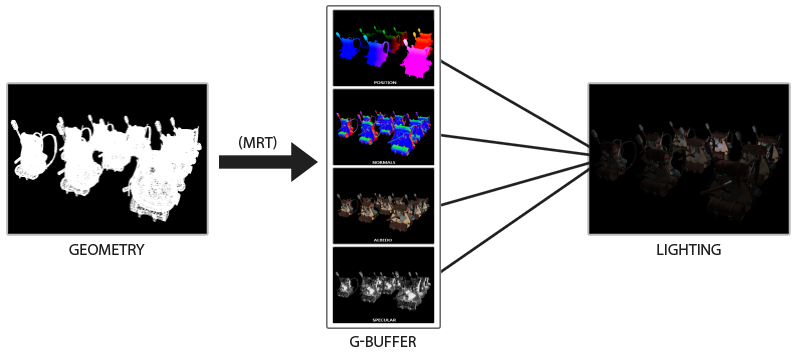
\includegraphics[width=.8\linewidth]{figures/deferred_pipeline_example.png}
   \caption{Schema generale della pipeline di deferred rendering da \cite{learnopengl}.}
   \label{fig:deferred-pipeline-example}
\end{figure}
Il motore sviluppato per questa tesi adotta una pipeline di tipo \emph{deferred}, in quanto offre una base più
flessibile per l'analisi delle prestazioni e per l'integrazione di tecniche di illuminazione avanzate.

\section{Physically Based Rendering (PBR)}
Il \emph{Physically Based Rendering} (PBR) mira a simulare il comportamento reale della luce e dei materiali,
basandosi su modelli fisici dell'interazione tra superfici e radiazione luminosa. A differenza dei modelli
tradizionali, che si affidano spesso a formule empiriche per ottenere un effetto visivamente piacevole, il PBR
definisce le proprietà dei materiali in modo coerente e indipendente dalle condizioni di illuminazione,
garantendo risultati più realistici e prevedibili.
Ogni materiale in un sistema PBR è descritto da un insieme di parametri fisici che ne determinano l'aspetto visivo.
I principali sono:
\begin{itemize}
   \item \textbf{Albedo} $A$: colore di base del materiale, senza effetti di illuminazione;
   \item \textbf{Roughness} $r$: rugosità microscopica della superficie, che determina la diffusione della luce speculare;
   \item \textbf{Metallic} $m$: indica se la superficie si comporta come un metallo (1) o un dielettrico (0);
   \item \textbf{Normal map} $\mathbf{N}$: mappa delle normali per simulare dettagli geometrici a livello micro;
   \item \textbf{Ambient Occlusion (AO)}: fattore che riduce l'intensità della luce ambientale in zone occluse.
\end{itemize}
\begin{figure}
   \centering
   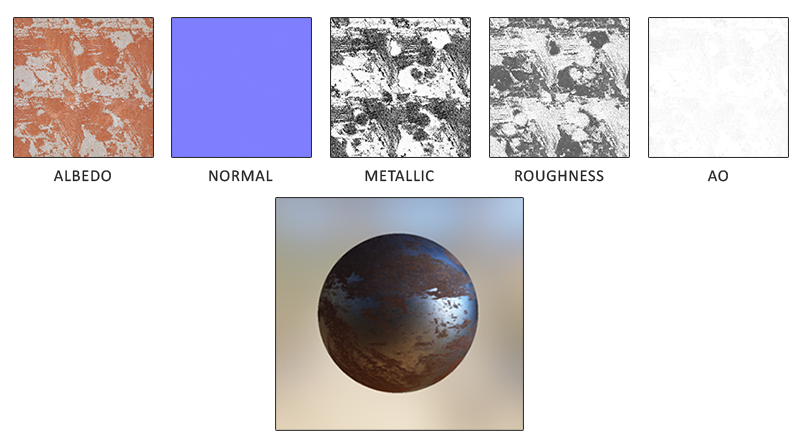
\includegraphics[width=.8\linewidth]{figures/pbr_material_example.png}
   \caption{Esempio di materiale PBR da \cite{learnopengl}.}
   \label{fig:pbr-material-example}
\end{figure}
Combinando questi parametri, il PBR consente di rappresentare in modo accurato una vasta gamma di materiali,
dai metalli lucidi ai tessuti ruvidi.

\section{Graphics API: OpenGL and Vulkan}
OpenGL e Vulkan rappresentano due approcci concettualmente diversi allo sviluppo di applicazioni grafiche.
OpenGL è un'API di livello alto che semplifica notevolmente la gestione della pipeline grafica: gran parte del lavoro
legato alla sincronizzazione delle risorse, alla gestione della memoria e alla compilazione dei comandi GPU è affidato
al driver. Questo approccio riduce la complessità dello sviluppo, consentendo di ottenere rapidamente risultati visivi,
ma limita il controllo del programmatore sulle prestazioni, soprattutto in scenari con molte luci e geometrie complesse.
OpenGL opera principalmente in modalità single-thread, affidando al driver l'organizzazione dei comandi su GPU, il che può
generare overhead significativi in applicazioni moderne e multithreaded.
Vulkan, al contrario, offre un modello di programmazione a basso livello, dove il programmatore ha il controllo diretto
sulla memoria, sui comandi e sulla sincronizzazione. La pipeline Vulkan richiede la definizione esplicita di tutti i
passaggi di rendering attraverso strutture come \texttt{Render Pass} e \texttt{Command Buffers}, e la gestione della 
sincronizzazione è completamente esplicita mediante \texttt{Semaphore} e \texttt{Fence}. Questo approccio riduce
l'overhead del driver e permette di sfruttare pienamente il multithreading della CPU, rendendo più efficienti
le applicazioni che devono gestire grandi quantità di oggetti e luci in scena. Allo stesso tempo, Vulkan richiede
una conoscenza approfondita dell'architettura hardware e della gestione delle risorse, aumentando la complessità
dello sviluppo rispetto a OpenGL.

\section{Librerie e Strumenti}
Il motore sviluppato utilizza un insieme di librerie open source per la gestione dell'infrastruttura di rendering
e delle funzionalità.
La combinazione di queste librerie ha permesso di ridurre il tempo di sviluppo e concentrarsi sulle differenze
architetturali tra OpenGL e Vulkan.
\begin{itemize}
   \item \textbf{GLFW}: fornisce un'interfaccia multipiattaforma per la creazione di finestre e la gestione dell'input.
      È utilizzata sia per il backend OpenGL che Vulkan;
   \item \textbf{GLAD}: gestisce il caricamento dinamico delle estensioni OpenGL;
   \item \textbf{Vulkan Memory Allocator (VMA)} e \textbf{vk-bootstrap}: semplificano la configurazione e la gestione della memoria
      Vulkan, riducendo la complessità di codice di inizializzazione;
   \item \textbf{glm}: libreria matematica per operazioni su vettori, matrici e trasformazioni 3D;
   \item \textbf{ImGui}: libreria per la costruzione di interfacce grafiche di debug e monitoraggio delle prestazioni in tempo reale;
   \item \textbf{stb\_image}: caricamento di texture in vari formati;
   \item \textbf{ASSIMP}: parsing dei modelli 3D in formato \texttt{.obj} e \texttt{.fbx}.
\end{itemize}

\section{Lavori Correlati}
Diversi studi e progetti hanno analizzato il confronto tra OpenGL e Vulkan, evidenziando vantaggi significativi di
Vulkan in termini di efficienza e parallelismo.
Il \emph{Khronos Group}, nelle specifiche di rilascio e nei documenti ufficiali, evidenzia come Vulkan sia progettata per
minimizzare l'overhead del driver e fornire prestazioni più prevedibili grazie a un controllo esplicito delle risorse e
dell'esecuzione dei comandi \cite{khronos_vulkan_spec,vulkan_overview,google_vulkan_lowoverhead}.
Sul fronte applicativo, motori come \emph{Unreal Engine 5} e \emph{Unity} hanno introdotto backend Vulkan per
ottimizzare la scalabilità su dispositivi moderni, mantenendo al contempo compatibilità con OpenGL su piattaforme legacy.

%----------------------------------------------------------------------------------------
\chapter{Requisiti ed Analisi}
\label{chap:analisi}
%----------------------------------------------------------------------------------------
\noindent
In questo capitolo vengono definiti i requisiti funzionali e non funzionali del motore di rendering 
e analizzate le motivazioni alla base delle scelte progettuali.
L’obiettivo è stabilire un quadro metodologico chiaro che guidi la progettazione e l’implementazione del sistema,
tenendo conto dei vincoli tecnici imposti dalle API e dall’hardware.
Lo sviluppo del motore di rendering oggetto di questo elaborato nasce con l'obiettivo di creare una piattaforma
sperimentale che permetta di confrontare in modo diretto le prestazioni e le differenze architetturali tra
OpenGL e Vulkan.
Dopo aver descritto le funzionalità attese e le caratteristiche qualitative del software,
si discutono i principali vincoli di progetto e le librerie adottate.
Il capitolo si conclude illustrando la strategia di valutazione delle prestazioni,
che costituisce la base per l’analisi comparativa tra OpenGL e Vulkan presentata nei capitoli successivi.
Questa fase di analisi ha costituito la base metodologica per orientare le scelte architetturali
presentate nei capitoli successivi.

\section{Requisiti funzionali}
Dal punto di vista funzionale, il motore deve essere in grado di gestire l'intero processo di rendering di una
scena tridimensionale complessa, fornendo un'infrastruttura flessibile per la sperimentazione con entrambe le API.
Il primo requisito riguarda la possibilità di selezionare, in fase di avvio, quale backend utilizzare tra OpenGL e
Vulkan. Tale scelta consente di confrontare le due pipeline in modo trasparente, mantenendo invariata la struttura
logica del motore e la scena visualizzata.

Il motore deve poi garantire la gestione completa delle risorse grafiche, tra cui modelli tridimensionali, texture e
shader. A tal fine, è stato previsto un sistema di caricamento e caching che consente di ridurre le operazioni ridondanti
e di ottimizzare la condivisione della memoria tra CPU e GPU. Il rendering della scena è realizzato attraverso una
pipeline di tipo \emph{deferred}, scelta per la sua maggiore efficienza nella gestione di un elevato numero di luci
dinamiche.

Un ulteriore requisito fondamentale riguarda il supporto al \emph{Physically Based Rendering (PBR)}, che permette
di ottenere una resa realistica dei materiali basandosi su parametri fisici. Il sistema deve inoltre consentire
l'utilizzo di differenti tipologie di luci con parametri configurabili dall'interfaccia di debug.

Nel backend Vulkan, il motore deve supportare la generazione multithread dei \texttt{command buffer}, così da sfruttare
in modo più efficiente i core della CPU. Questa caratteristica è essenziale per valutare i benefici del parallelismo
offerto da Vulkan rispetto al modello single-thread di OpenGL. Infine, il motore deve includere una telecamera
controllabile in tempo reale e un'interfaccia grafica basata su ImGui per la visualizzazione delle statistiche di
esecuzione e dei parametri di scena.

\section{Requisiti non-funzionali}
Oltre alle funzionalità previste, il progetto deve rispettare una serie di requisiti non funzionali che ne
determinano la qualità complessiva. L'aspetto più rilevante è quello prestazionale: il motore deve essere in grado
di mantenere un frame rate stabile e prevedibile, anche in presenza di scene complesse. L'efficienza del codice e
la riduzione dell'overhead di CPU sono obiettivi primari, soprattutto nella versione Vulkan.

Un altro requisito riguarda la portabilità. Il sistema deve poter essere compilato ed eseguito sia su Windows che su
Linux, senza modifiche sostanziali al codice sorgente. Questo ha orientato la scelta di librerie multipiattaforma
come GLFW per la gestione delle finestre e dell'input, e glm per le operazioni matematiche tridimensionali.
La manutenibilità è stata garantita attraverso una struttura modulare del codice, che separa nettamente la logica di
rendering dalle altre componenti, come la gestione delle risorse o la GUI. Tale separazione consente di estendere il
motore in futuro con nuove tecniche di shading o ulteriori passaggi di rendering, senza introdurre dipendenze
circolari o modifiche invasive.

L'affidabilità rappresenta un ulteriore requisito importante. In particolare, è necessario assicurare che le risorse
allocate sulla GPU vengano correttamente rilasciate al termine dell'esecuzione, prevenendo perdite di memoria o crash.
La presenza dell'interfaccia di debug consente inoltre di monitorare in tempo reale l'utilizzo delle risorse e il
tempo di esecuzione dei frame, migliorando la tracciabilità e la diagnosi dei colli di bottiglia.

\section{Vincoli di progetto}
Il progetto è stato sviluppato nel rispetto di alcuni vincoli tecnici legati sia alla piattaforma hardware sia alle
librerie disponibili. Il linguaggio scelto è \textbf{C++23}, che offre un buon compromesso tra efficienza,
astrazione e modernità, consentendo l'utilizzo di costrutti avanzati come le \emph{smart pointer} e le
\emph{range-based loops}. Le API grafiche target sono OpenGL 4.6 e Vulkan 1.4, in modo da garantire compatibilità
con la maggior parte delle GPU moderne.

Dal punto di vista hardware, i test sono stati condotti su una configurazione dotata di processore multi-core e GPU
di fascia medio-alta compatibile con le specifiche Vulkan. È importante sottolineare che le prestazioni osservate
dipendono fortemente dal sistema su cui vengono eseguiti i test, motivo per cui i risultati discussi nei capitoli
successivi si riferiscono a un ambiente controllato e costante.

Il motore si appoggia a un insieme di librerie open source per ridurre il tempo di sviluppo e migliorare la stabilità
del codice. Tra queste rientrano GLFW per la creazione delle finestre, GLAD per il caricamento dinamico delle estensioni
OpenGL, Vulkan Memory Allocator e vk-bootstrap per la gestione semplificata delle risorse Vulkan, ImGui per
l'interfaccia di debug, glm per le operazioni matematiche e ASSIMP per il caricamento dei modelli tridimensionali.
Il sistema di build adottato è CMake, che garantisce la compatibilità con ambienti di sviluppo diversi.

Per delimitare il campo di studio, sono stati esclusi elementi non essenziali all'obiettivo sperimentale, come il
ray tracing, le ombre dinamiche avanzate o il supporto a dispositivi mobili. La ricerca si concentra esclusivamente
sulle differenze di prestazioni e di gestione delle risorse tra le due API, in un contesto di rendering differito
tradizionale.

\section{Strategia di Valutazione}
La valutazione delle prestazioni rappresenta una parte fondamentale di questo lavoro. La strategia adottata prevede
una serie di test ripetibili e controllati, condotti su una scena di riferimento comune: la cattedrale di
Sponza~\cite{sponza_original,sponza_intel2022}, ampiamente utilizzata come benchmark nella letteratura di grafica
computazionale. I test vengono eseguiti con configurazioni identiche per i due backend, variando il numero di luci,
la complessità della scena e il livello di parallelismo della CPU.

Le metriche considerate includono il tempo medio per frame, il frame rate e l'utilizzo medio della CPU e della GPU.
I dati vengono raccolti tramite un sistema di monitoraggio integrato nell'interfaccia di debug, che consente la
registrazione automatica dei risultati per l'analisi successiva.

Ciascun test viene ripetuto più volte per ridurre l'impatto di fattori esterni, come i processi di sistema o
l'oscillazione della frequenza della GPU. I risultati vengono poi confrontati e discussi nel
Capitolo~\ref{chap:valutazione}, dove vengono analizzate le differenze di comportamento tra OpenGL e Vulkan in termini
di efficienza, scalabilità e prevedibilità delle prestazioni.

%----------------------------------------------------------------------------------------
\chapter{Progettazione e Architettura del Sistema}
\label{chap:design}
%----------------------------------------------------------------------------------------

\section{Panoramica del Sistema}

\section{Progettazione Orientata agli Oggetti}

\section{Architettura del Motore di Rendering}

\section{Pipeline di Deferred Rendering}

\section{Gestione delle Risorse}

%----------------------------------------------------------------------------------------
\chapter{Implementazione}
\label{chap:implementazione}
%----------------------------------------------------------------------------------------

\section{Struttura del Codice}

\section{Componenti Principali}

\section{Sistema di Materiali PBR}

\section{Simulazione di Particelle}

\section{Interfaccia Grafica per le Prestazioni}

%----------------------------------------------------------------------------------------
\chapter{Valutazione delle Prestazioni}
\label{chap:valutazione}
%----------------------------------------------------------------------------------------

\section{Configurazione Sperimentale}

\section{Risultati}

\section{Discussione}

%----------------------------------------------------------------------------------------
\chapterWithoutNumber{Conclusioni e Sviluppi Futuri}
\label{chap:conclusioni}
%----------------------------------------------------------------------------------------

\paragraph{Sintesi del Lavoro}

\paragraph{Risultati Principali}

\paragraph{Limitazioni del Lavoro}

\paragraph{Sviluppi Futuri}

% End of thesis
\backmatter

\nocite{*}

\bibliographystyle{alpha}
\bibliography{bibliography}

% TODO: Write acknowledgements (optional)
\begin{acknowledgements}
   Optional. Max 1 page.
\end{acknowledgements}

\end{document}
